Have you ever been frustrated at the price of gas? Cars are an integral part of most people’s lives, especially in the United States, so it makes sense that people feel strongly about the price of gas. Gas is not the only product affected by the price of crude oil, but it is the one that most people probably think of when they hear “crude oil.” Crude oil is one of the most important commodities in modern society and its price is tied to a large number of factors. Oil is collected from many locations around the world and whenever major events happen in these locations, it can shift oil production rates which in turn affects the price of oil. This report will explain how this crude oil price data was collected, what it actually means, how it can be visualized, and how trends in the data can be explained by real-world events with a specific example.


\begin{figure}
  \centering
  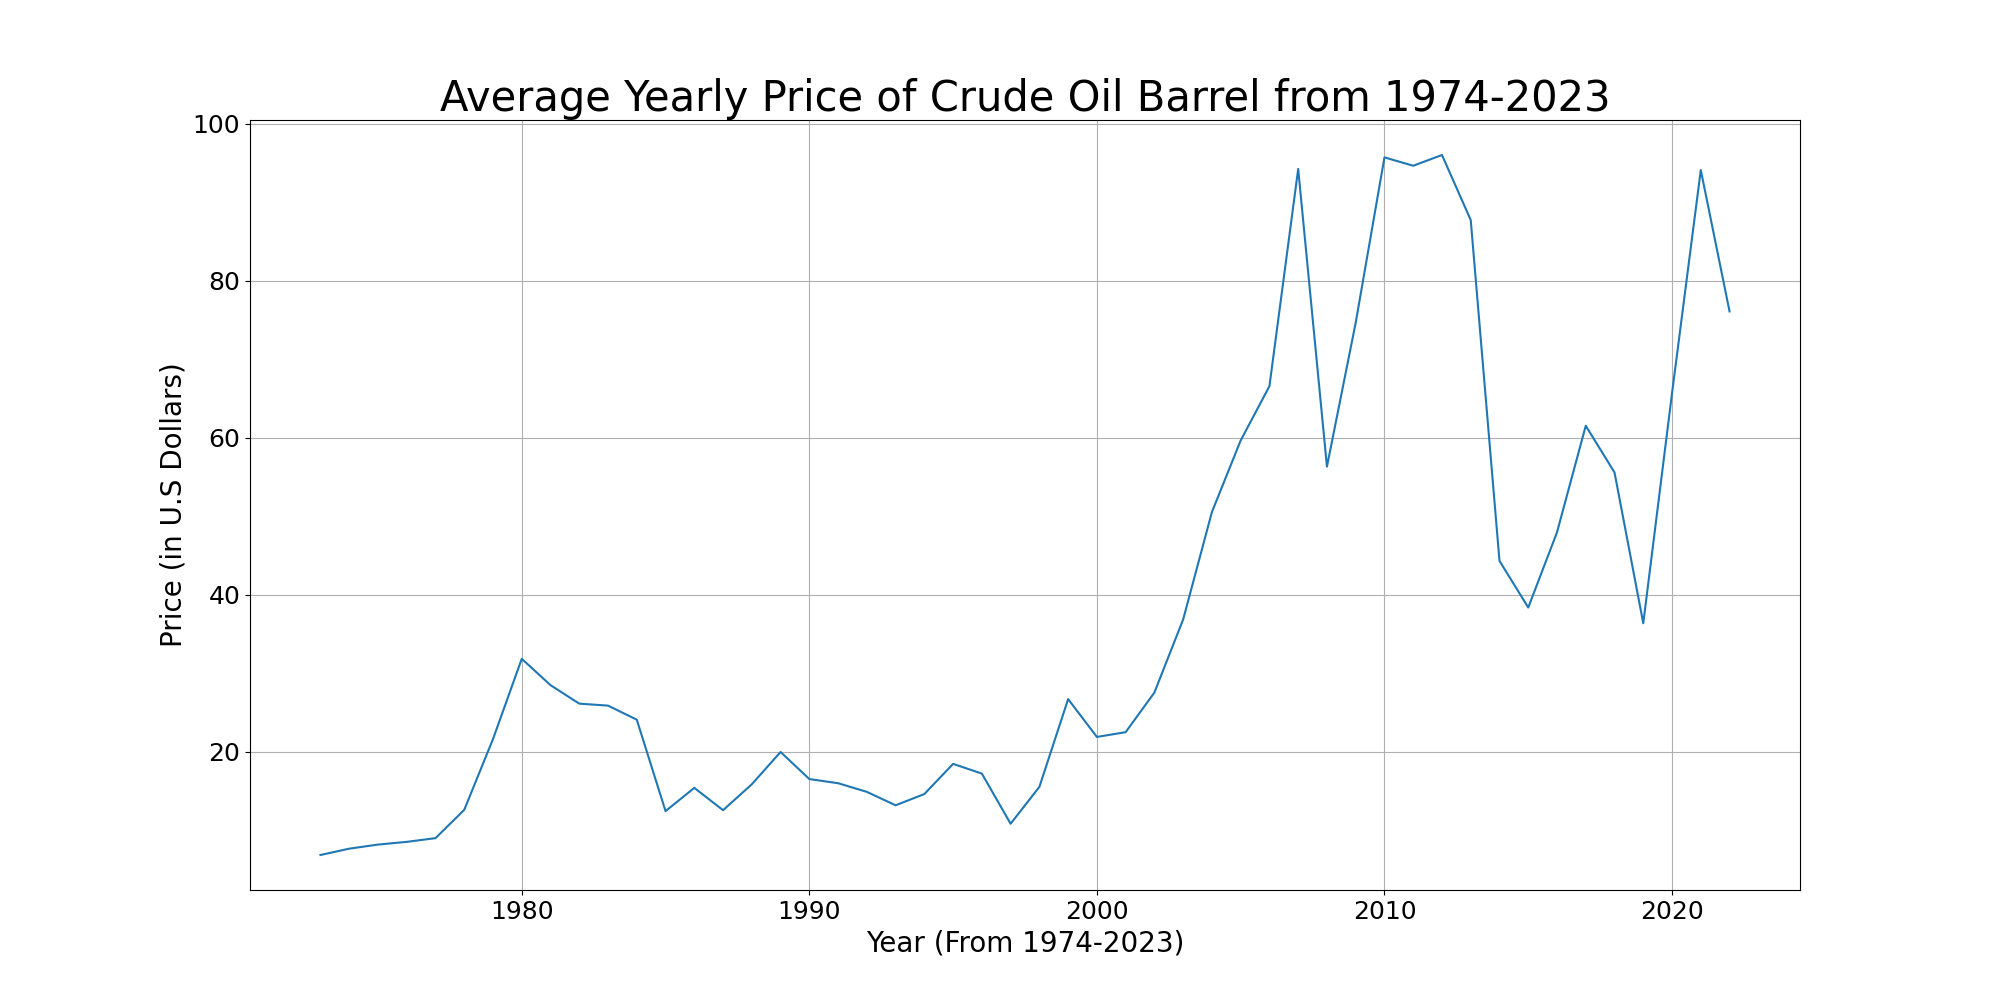
\includegraphics[width=1.0\textwidth]{OilPrice1.png}
  \caption{This is the graph of average Crude oil barrel prices. It was made using the modified lists of data and pylab}
 
  \label{fig:AverageOilPricePlot}
\end{figure}


